% !TEX root = ../main.tex
\newpage
% Раздел 2
\section{Теоретические сведения}\label{sec:razd2} % Теоретические сведения

\subsection{Языки программирования и библиотеки}

В качестве основного языка был выбран Python -- высокоуровневый интерпретируемый
язык программирования общего назначения с динамической типизацией
данных \cite{python}.

К достоинствам Python можно отнести:
\begin{itemize}
    \item Язык является интерпретируемым (не требует компиляции), что повышает
    производительность разработчика при написании и отладке программного кода.
    \item Кроссплатформенность. Основной интерпретатор языка (CPython)
    реализован для большинства активно используемых платформ, что позволяет
    использовать один и тот же код на любой системе.
    \item Имеется большая стандартная библиотека и множество пользовательских
    модулей, находящихся в открытом доступе.
\end{itemize}

Основные недостатки языка:
\begin{itemize}
    \item Низкое быстродействие;
    \item Не слишком удачная поддержка многопоточности.
\end{itemize}

Реализуемая программа состоит из двух частей:
\begin{enumerate}
    \item Графический интерфейс;
    \item Подсистема шифрования.
\end{enumerate}

Графический интерфейс программы был реализован с использованием библиотеки Qt5
и ее привязки к Python -- PyQt5.

Несмотря на особенности выполняемой задачи (шифрование текстовых документов),
в общем случае шифрование должно выполняться эффективно по времени.
Из-за низкой скорости выполнения кода использовать Python для реализации криптографических
методов, в частности алгоритмов шифрования, является нежелательным.
Для повышения производительности рассмотрено две альтернативы: использовать язык C (стандарт C99) или
язык ассемблера. В разделе \ref{sec:razd3} приведен краткий анализ реализаций
алгоритмов шифрования на языке ассемблера и C.

\newpage
\subsection{Алгоритмы шифрования}

В проекте на данный момент реализовано два алгоритма шифрования:
FEAL-4 и Blowfish. Выбор первого обусловлен простотой реализации и
довольно высокой скоростью работы, несмотря на невысокую криптографическую
стойкость: шифр может быть взломан по пяти подобранным исходным блокам
с использованием линейного криптоанализа \cite{feal-attack}.

Алгоритм Blowfish является безопасным незапатентованным свободным для
использования шифром. На данный момент, в отличие от FEAL-4, не существует
эффективных методов взлома шифра Blowfish.

Алгоритм FEAL (Fast data Encipherment ALgorithm) был разработан криптографами
Акихиро Симидзу (Akihiro Shimizu) и Сёдзи Миягути (Shoji Miyaguchi) из
японской компании NTT в 1987 г. \cite[стр. 206]{panasenko}.

Разработчики алгоритма продвигали FEAL как потенциальную замену стандарта
шифрования DES -- по их мнению, FEAL-4 (число в названии обозначает количество
раундов алгоритма) предлагал более быстрое шифрование без потери его качества.
Кроме того, в FEAL отсутствуют табличные замены, поэтому реализация алгоритма
не требует дополнительной энергонезависимой памяти для хранения таблиц.

На рисунке \ref{fig:feal-nx-structure} представлена структура общего варианта
алгоритма FEAL -- FEAL-NX -- вместе с функцией расширения ключа. В упрощенном
варианте алгоритма FEAL-4 функция расширения не используется, поэтому рассмотрена
не будет.

Алгоритм FEAL-4 имеет структуру сети Фейстеля:
в каждом раунде выполняется обработка правого 32-битного подблока функцией
$F(R,k_{16})$, где $R$ -- правый подблок данных, $k_{16}$ -- 16-битное значение
ключа раунда. Результат обработки накладывается на левой подблок операцией XOR.
Перед первым раундом выполняется операция $XOR$ блока шифруемых данных с
ключом, а также аналогичное наложение левого подблока на правый.
После финального раунда алгоритма также производятся те же действия:
наложение левого блока на правый и сложение с ключом.
Расшифрование выполняется аналогично, но 16-битовые подключи подставляются
в обратном порядке.

\noindent
\begin{minipage}{\linewidth}
  \centering
  \vspace{3.5mm}
  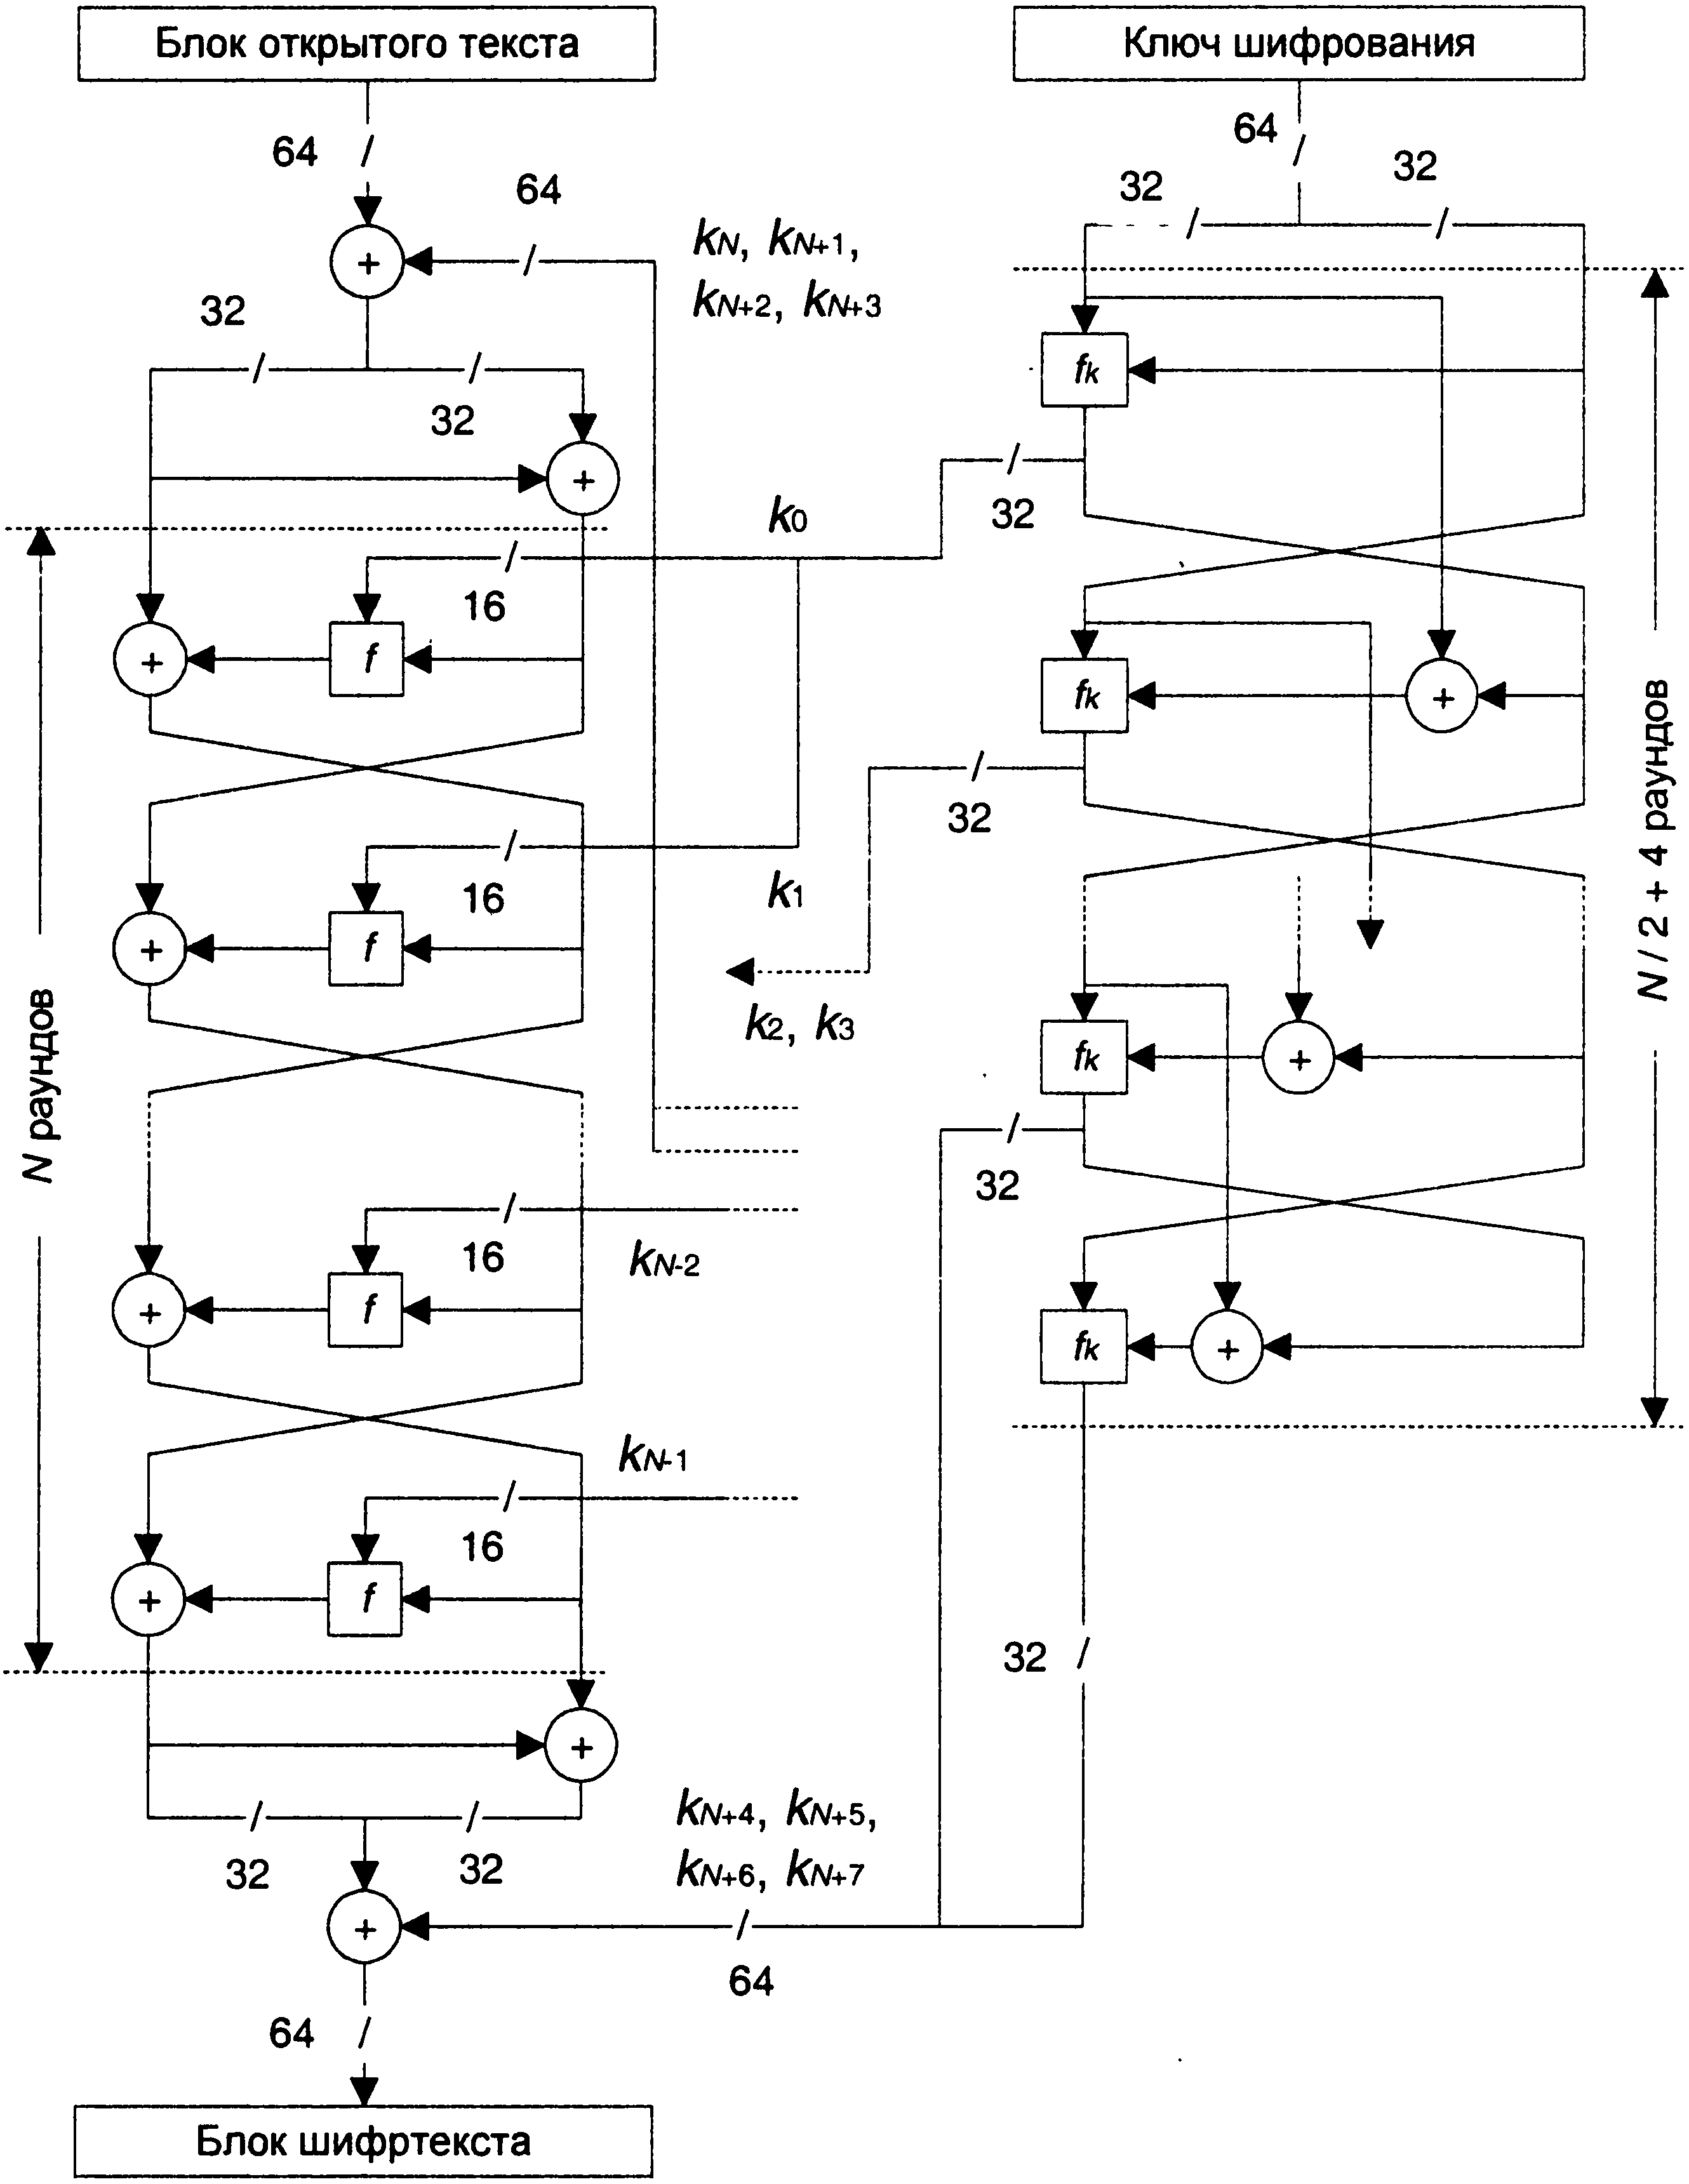
\includegraphics[scale=0.2]{./pics/feal-nx-structure.png}
  \captionof{figure}{Структура алгоритма FEAL-NX.}\label{fig:feal-nx-structure}
  \vspace{3.5mm}
\end{minipage}

Структура функции $F$ представлена на рисунке \ref{fig:feal-nx-f}.
В ней используются лишь три вида преобразований: операция $XOR$,
функции $S_0$ и $S_1$, которые можно описать следующим образом:
\begin{align*}
  S_0 = & \text{ROL}_2((x+y)\text{mod}2^8), \\
  S_1 = & \text{ROL}_2((x+y+1)\text{mod}2^8),
\end{align*}
где $\text{ROL}_2$ -- операция циклического сдвига влево на два разряда.

\noindent
\begin{minipage}{\linewidth}
  \centering
  \vspace{3.5mm}
  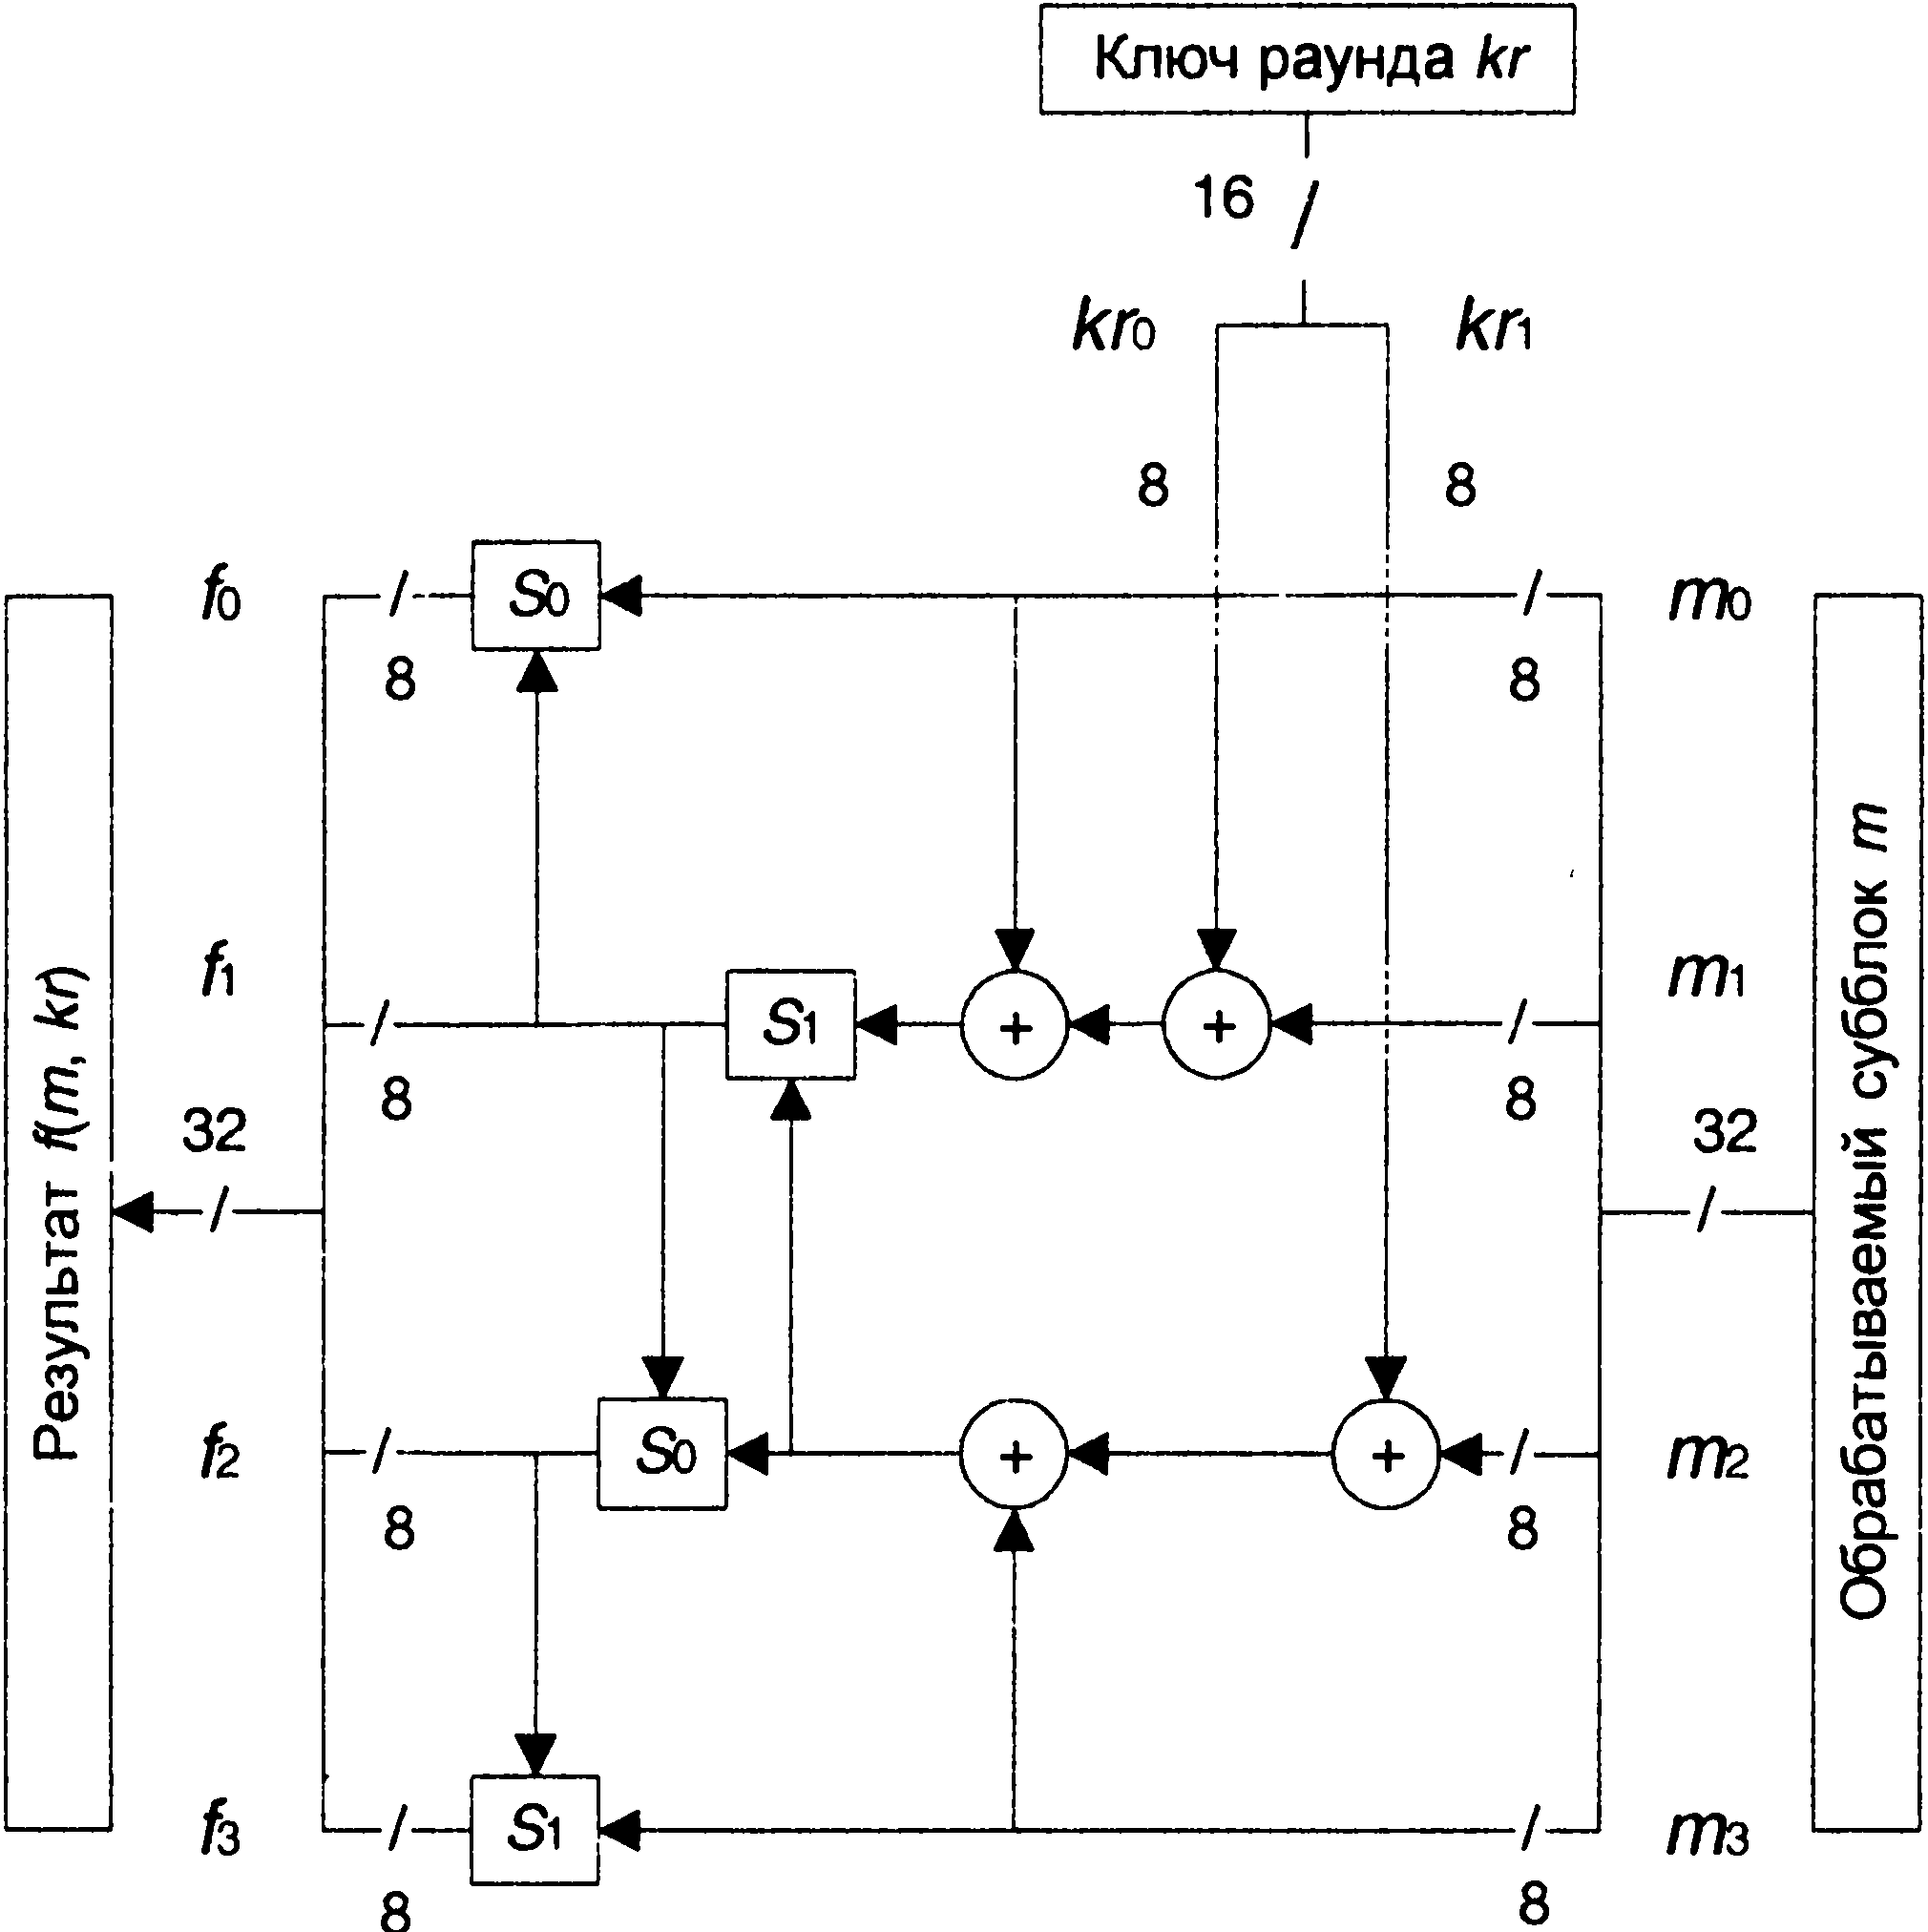
\includegraphics[scale=0.2]{./pics/feal-nx-f.png}
  \captionof{figure}{Функция $F$ алгоритма FEAL-4.}\label{fig:feal-nx-f}
  \vspace{3.5mm}
\end{minipage}

Алгоритм FEAL-4, изначально предлагавшийся в качестве замены стандарта DES,
оказался весьма нестоек к различным видам криптоанализа. Та же участь постигла
и алгоритм FEAL-8. Алгоритмы FEAL-16, FEAL-32 и т. д. оказались существенно
более стойкими за счет большего количества раундов. Однако скорость их работы
оказалась ниже скорости алгоритма DES. Поэтому, как стандарт шифрования,
алгоритм FEAL не состоялся.

Алгоритм Blowfish разработан Брюсом Шнайером в 1994 г. также в качестве
замены DES \cite[стр. 118]{panasenko}.
Алгоритм оказался весьма удачным и приобрел широкую популярность. Он очень широко реализован в различных
средствах защиты информации.

Blowfish, как и FEAL-4, шифрует данные 64-битными блоками, однако размер
ключа может варьироваться от 32 до 448 бит. Алгоритм также представляет
собой сеть Фейстеля, его структура приведена на рисунке \ref{fig:blowfish-structure}.

\noindent
\begin{minipage}{\linewidth}
  \centering
  \vspace{3.5mm}
  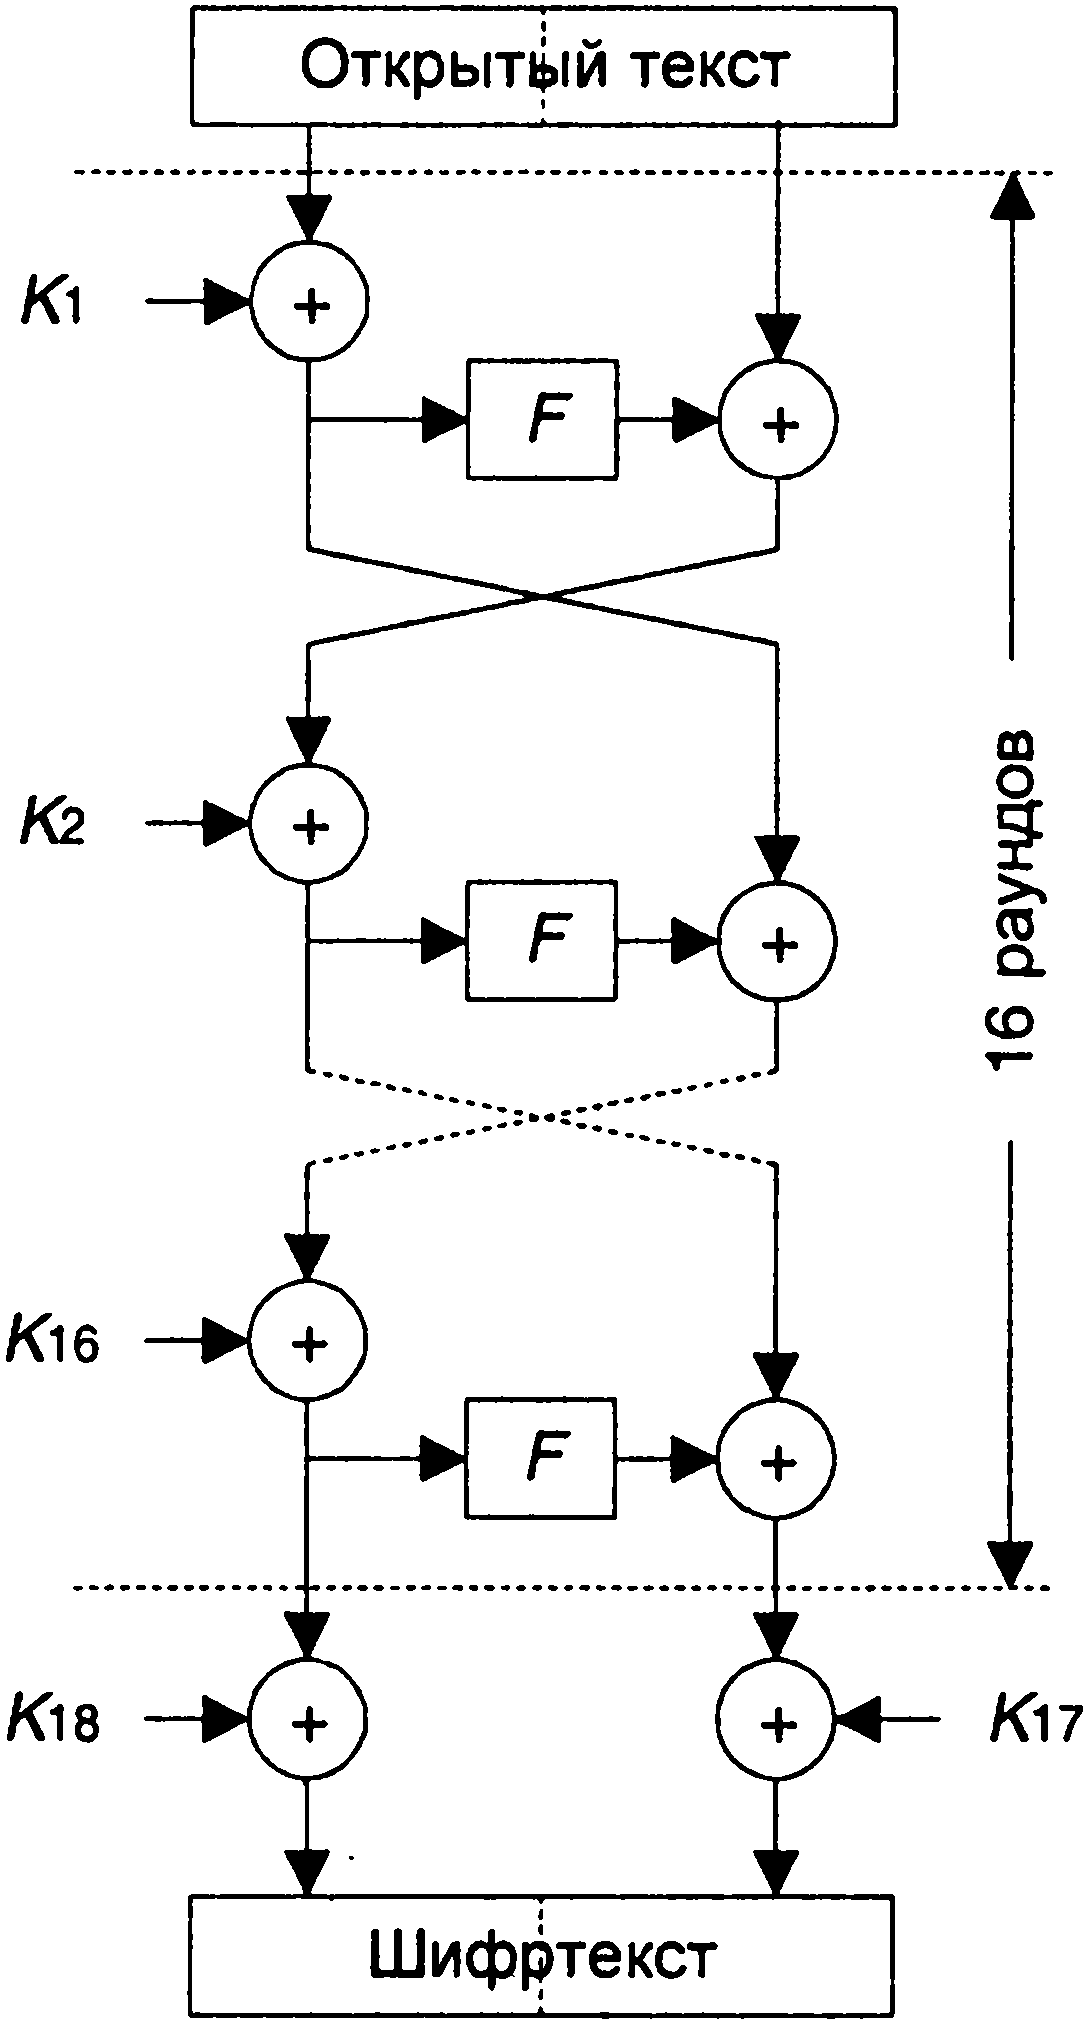
\includegraphics[scale=0.2]{./pics/blowfish-structure.png}
  \captionof{figure}{Структура алгоритма Blowfish.}\label{fig:blowfish-structure}
  \vspace{3.5mm}
\end{minipage}

Шифрование данных выполняется в 16 раундов, в каждом из которых над левым
32-битным подблоком данных производятся следующие действия \cite{blowfish}:
\begin{enumerate}
  \item Значение подблока складывается с ключом i-го раунда $K_i$ операцией
  $XOR$, результат операции становится новым значением подблока.
  \item Подблок обрабатывается функцией $F$. Результат обработки накладывается
  на правый подблок операцией $XOR$.
  \item Подблоки меняются местами во всех раундах, кроме последнего.
\end{enumerate}

После 16 раундов выполняется наложение на подблоки еще двух подключей:
$K_{17}$ и $K_{18}$ складываются операцией $XOR$ с правым и левым
подблоками соответственно.

Функция $F$ (рисунок \ref{fig:blowfish-f}) обрабатывает подблок следующим образом:
\begin{enumerate}
  \item 32-битное входное значение делится на четыре фрагмента по восемь битов,
  каждый из которых является индексом соответствующих таблиц замен $S_1..S_4$.
  \item Значения из таблиц $S_1$ и $S_2$ складываются по модулю $2^{32}$.
  \item Полученное значение складывается операцией $XOR$ со значением из $S_3$.
  \item Полученное значение складывается по модулю $2^{32}$ со значением из $S_4$.
\end{enumerate}

Расшифрование выполняется аналогично шифрованию, но ключи $K_1..K_{18}$
используются в обратном порядке.

\noindent
\begin{minipage}{\linewidth}
  \centering
  \vspace{3.5mm}
  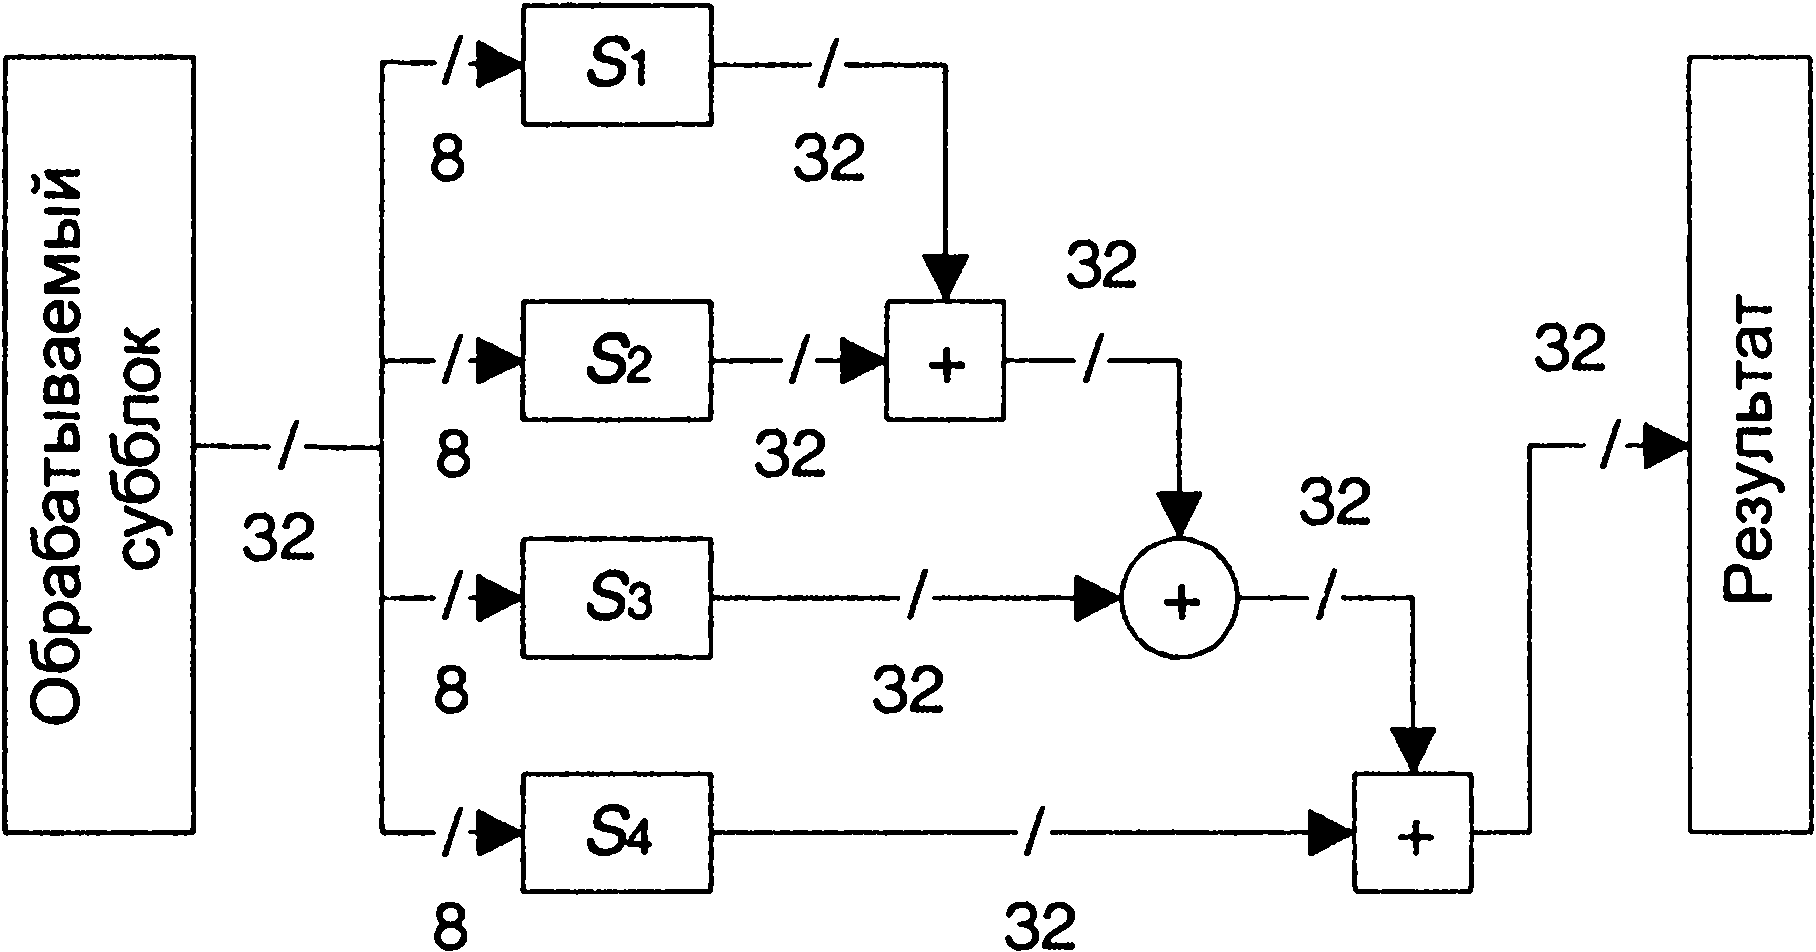
\includegraphics[scale=0.2]{./pics/blowfish-f.png}
  \captionof{figure}{Функция $F$ алгоритма Blowfish.}\label{fig:blowfish-f}
  \vspace{3.5mm}
\end{minipage}

В отличие от FEAL-4, перед шифрованием алгоритмом Blowfish необходимо
сгенерировать раундовые 32-битные ключи $K_1..K_{18}$ и четыре таблицы
замены $S_1..S_4$. Каждая таблица замены содержит 256 32-битных значений.

Процедура расширения ключа состоит из следующих шагов:
\begin{enumerate}
  \item Исходные значения ключей раундов и табилиц замен инициализируются
  псевдослучайно строкой, в качестве которой используется шестнадцатеричная
  запись дробной части числа $\pi$. Исходные значения ключей и таблиц можно
  найти в приложении В.
  \item Операцией $XOR$ на $K_1$ накладываются первые 32-бита ключа шифрования,
  на $K_2$ -- следующие 32 бита и т.д. до $K_{18}$. Ключ шифрования накладывается
  циклически, если используется более короткий ключ шифрования, чем необходимо
  для наложения на $K_1$..$K_{18}$.
  \item С использованием полученных ключей раундом и таблиц замен выполняется
  шифрование алгоритмом Blowfish блока данных, состоящего из 64 нулевых битов.
  Результат становится новым значением ключей $K_1$ и $K_2$.
  \item Используя измененные значения ключей $K_1$ и $K_2$, шифруется результат,
  полученный на предыдущем этапе. В результате получаются новые значения ключей
  $K_3$ и $K_4$.
  \item Шифрование выполняется до тех пор, пока новыми значениями не будут
  заполнены все ключи раундов и таблицы замен.
\end{enumerate}

Особенностью алгоритма Blowfish является то, что он не годится
для применения в случаях, где требуется частая смена ключей. Процедура
расширения ключа является достаточно ресурсоемкой, поэтому одно из достоинств
алгоритма Blowfish -- достаточно высокая скорость шифрования -- проявляется
только в тех случаях, если на одном ключе шифруется достаточно большой объем
информации. И наоборот, если менять ключ после каждого из шифруемых блоков,
скорость алгоритма становится катастрофически низкой именно из-за необходимости
каждый раз выполнять расширения ключа.

Явные достоинства и отсутствие критичных недостатков предопределили
широкое использование алгоритма Blowfish.

\subsection{Хранение данных}

Для хранения зашифрованных данных необходимо обеспечить:
\begin{itemize}
    \item Целостность данных;
    \item Поддержка нескольких алгоритмов шифрования и хэширования;
\end{itemize}

Для хранения зашифрованных данных была спроектирована структура файла,
включающая в себя:
\begin{enumerate}
  \item Заголовок.
  \begin{enumerate}
    \item Магическое число (сигнатура) -- 4 байта : \verb"'tfe', 0x42".
    \item Используемый алгоритм -- 1 байт.
    \item Используемая функция хэширования -- 1 байт.
    \item Отступ до зашифрованных данных от начала заголовка -- 2 байта.
    \item Размер исходных зашифрованных данных -- 8 байт.
  \end{enumerate}
  \item Преамбула.
  \begin{enumerate}
    \item Хэш первых 512 байт исходных данных -- размер зависит от
    используемой функции хэширования.
    \item Соль для пароля -- 16 байт.
  \end{enumerate}
  \item Зашифрованные данные.
\end{enumerate}

Используемый алгоритм и функция хэширования являются номерами
в таблицах функций алгоритмов и функций хэширования. На данный
момент реализована поддержка следующих функций:
\begin{itemize}
  \item Функции шифрования:
  \begin{enumerate}
    \item FEAL-4;
    \item Blowfish;
  \end{enumerate}
  \item Функции хэширования:
  \begin{enumerate}
    \item MD5;
  \end{enumerate}
\end{itemize}

При использовании блочного шифра в режиме EBC необходимо дополнить исходные
данные, чтобы их размер стал кратен размеру блока. В реализации последний
блок данных дополняется необходимым количеством байтов со значением 0x42.
При дешифровании лишние байты отрезаются, так как известен размер
зашифрованных данных.

Формат позовляет хранить зашифрованные данные любого типа,
есть возможность проверить полученные после расшифрования данные
на соответствие исходным данным (то есть проверить был ли использован
правильный ключ при расшифровании).

Однако такой формат может быть контейнером только для одного файла.
Отсутствует встроенная поддержка сжатия данных и возможность восстановить
тип исходного файла.

Несмотря на перечисленные ограничения, спроектированный формат зашифрованного файла
подойдет для использования в разрабатываемом программном средстве.

\subsection{Проектирование интерфейса}

Графический пользовательский интерфейс программы должен выглядеть
как обычный текстовый редактор (рисунок \ref{fig:generic-text-editor}).
В рамках рассматриваемой задачи интерфейс должен предоставлять
пользователю следующие функции:
\begin{itemize}
    \item Редактирование текстовых файлов;
    \item Шифрование текстовых файлов;
    \item Базовые настройки текстового редактора (внешний вид, шрифт);
    \item Основные настройки шифрования.
\end{itemize}

\noindent
\begin{minipage}{\linewidth}
  \centering
  \vspace{3.5mm}
  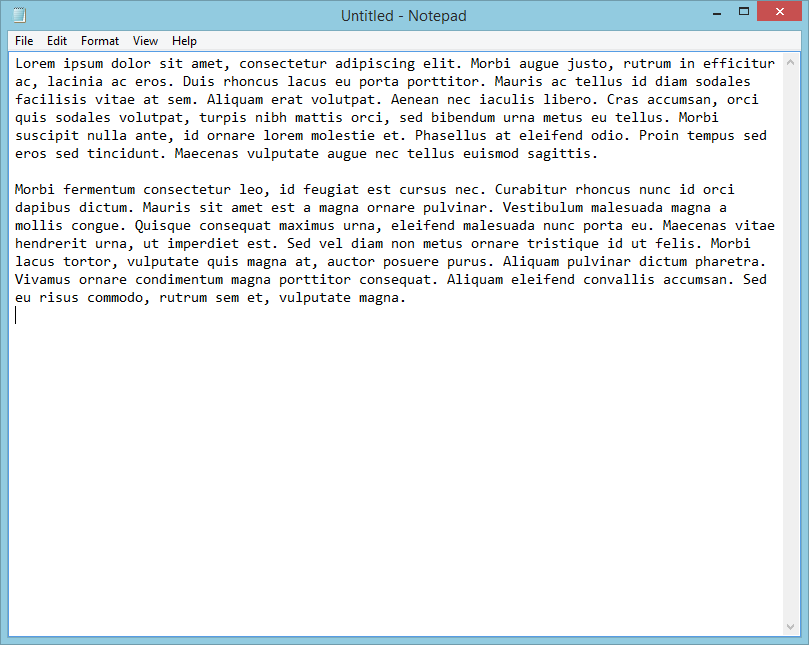
\includegraphics[scale=0.6]{./pics/generic-text-editor.png}
  \captionof{figure}{Интерфейс обычного текстового редактора.}\label{fig:generic-text-editor}
  \vspace{3.5mm}
\end{minipage}
